\documentclass[xcolor={dvipsnames}]{beamer}

\usetheme{Malmoe}
\usecolortheme{seagull}
\usepackage[]{natbib}
\usepackage{textpos}
\usepackage{amsmath, amssymb, bm}
\usepackage{multirow}
\usepackage{framed}
\usepackage{schemata}
\setbeamertemplate{navigation symbols}{}
\usepackage[english]{babel}
\usepackage{animate}
\usepackage{graphics}
\usepackage{fontawesome}


\definecolor{lightblue}{rgb}{0.145,0.6666,1} % Defines the color used for content box headers
\definecolor{Red}{rgb}{0.9,0.15,0}
\definecolor{Blue}{RGB}{55,126,184}
\definecolor{Green}{RGB}{77,175,74}
\definecolor{White}{RGB}{255,255,255}
\definecolor{Lightgray}{rgb}{0.86,0.86,0.86}

\setbeamertemplate{footline}
{
	\leavevmode%
	\hbox{%
		\begin{beamercolorbox}[wd=.50\paperwidth,ht=2.25ex,dp=1ex,center]{author in head/foot}%
			\usebeamerfont{author in head/foot}\insertshortauthor%% \beamer@ifempty{\insertshortinstitute}{}{(\insertshortinstitute)}
		\end{beamercolorbox}%
%		\hskip2pt%
		\begin{beamercolorbox}[wd=.50\paperwidth,ht=2.25ex,dp=1ex,center]{title in head/foot}%
			\usebeamerfont{title in head/foot}\insertshorttitle~~~~~~~~~~~~~~~~~~~~~~~~~~\insertframenumber
		\end{beamercolorbox}%
	}%
	\vskip0pt%
}
\makeatother

\title[Macro patterns of aging]{
	\small{\textsl{BSPS 2017}}\\$\,$\\$\,$}

\subtitle{\large{\textsc{Macro patterns in the evolution of human aging}}\\$\,$\\}


\author[IBSPS. Riffe \& Aburto,  2017]
{
	\vspace{-0.5cm}
	\texorpdfstring{
		\begin{columns}
			\column{.9\linewidth}
			\centering
			\normalsize{ Tim Riffe \& Jos\'{e} Manuel Aburto}\\
			$\,$\\
			\begin{center}			
			
\includegraphics[scale=0.15]{Figures/logos.pdf}     
			\end{center}
		\end{columns}
	}
	{Tim Riffe \& Jos\'{e} Manuel Aburto}
}

\date[]{8$^{\textrm{th}}$ September 2017}

\beamertemplatenavigationsymbolsempty
\begin{document}


\begin{frame}[plain]
	\titlepage
\end{frame}
%%%%%%%%%%%%%%%%%%%%%%%%%%%%%%%%%%%%%%%%%%%%%%%%%%%%%%%%%%%%%%%%%%%%%%%%%
%%%%%%%%%%%%%%%%%%%%%%%%%%%%%%%%%%%%%%%%%%%%%%%%%%%%%%%%%%%%%%%%%%%%%%%%%
\section{Introduction}

%%%%%%%%%%%%%%%%%%%%%%%%%%%%%%%%%%%%%%%%%%%%%%%%%%%%%%%%%%%%%%%%%%%%%%%%%
\begin{frame}\frametitle{Background}
\Large{
		\begin{itemize}
		
		\item<1-> \textbf{Life expectancy} at birth ($e_0$) is the most used indicator.
		
		\item<2-> Demographers also use \textbf{modal} or  \textbf{median} age at death.
		
		\item<3-> They \textbf{conceal variation of lifespans} and other aspects of the age at death distribution.
			
		
		\end{itemize} }

\end{frame}
	\begin{center}
		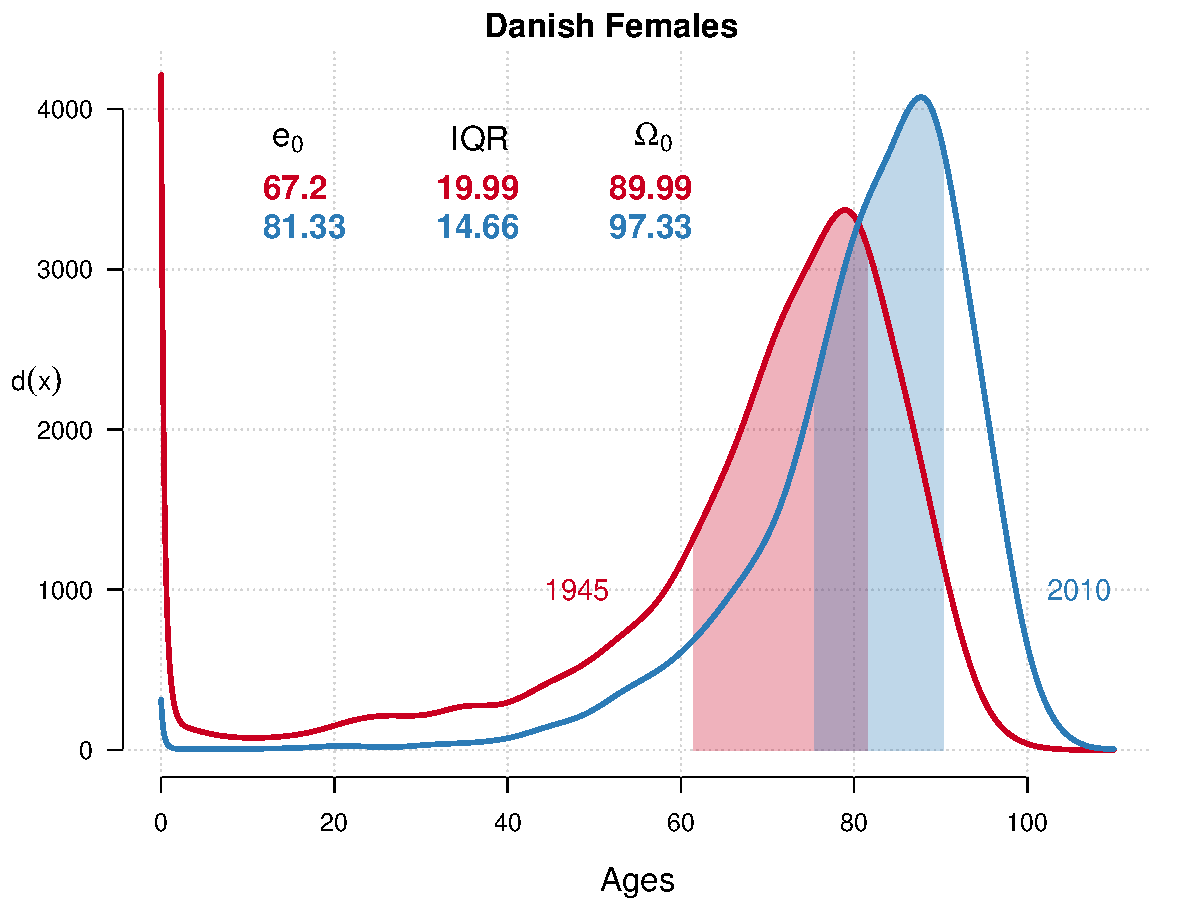
\includegraphics[scale=.52]{Figures/Fig0}
				\end{center}
				
			

\section{Formulae}

\begin{frame}\frametitle{Key formulas}
\large{
Consider the conditional death distribution

\begin{equation*}
f(y \mid a)= \frac{1}{\ell (a)} \textcolor{red}{\mu (a + y)} \textcolor{blue}{\ell (a + y)}
\end{equation*}
\pause

\textcolor{red}{$\mu(a)\longrightarrow $ force of mortality at age $a$} \\
\textcolor{blue}{$\ell (a)\longrightarrow $ survivorship to age $a$}
\linebreak

\pause

\textbf{Key point: $f(y \mid a) \longrightarrow $ probability of surviving to and dying at age 
$a+y$ given survival to age $a$.}}

\end{frame}

\begin{frame}
\large{
Remaining life expectancy conditional on survival to age $a$ is 

\begin{equation*}
e(a)= \frac{1}{\ell (a)} \int_0^\infty \ell (a + y)dy
\end{equation*}
\linebreak

\textbf{The conditional deaths distribution can be described by its moments about $e(a)$}}
\end{frame}


\begin{frame}
\large{
Moment generator function defined as

\begin{equation*}
\eta_n(y \mid a) = \int_{y=0}^\infty (y - e(a))^n f(y \mid a) dy
\end{equation*}
\linebreak

\pause
\textcolor{red} {Variance $\longrightarrow \sigma^2(y \mid a) = \eta_2(y \mid a)$ }
\linebreak

\pause
\textcolor{Orchid} {Skewness $\longrightarrow Skew(y \mid a) = \frac{ \eta_3(y \mid a)}{\sigma^2(y \mid a)} $ }
\linebreak

\pause
\textcolor{NavyBlue} {Kurtosis $\longrightarrow Kurt(y \mid a) = \frac{ \eta_4(y \mid a)}{\sigma^3(y \mid a) - 3} $ }}


\begin{center}
$\vdots$
\end{center} 

\end{frame}






\section{Illustration}
\begin{frame}
		
			\begin{center}
		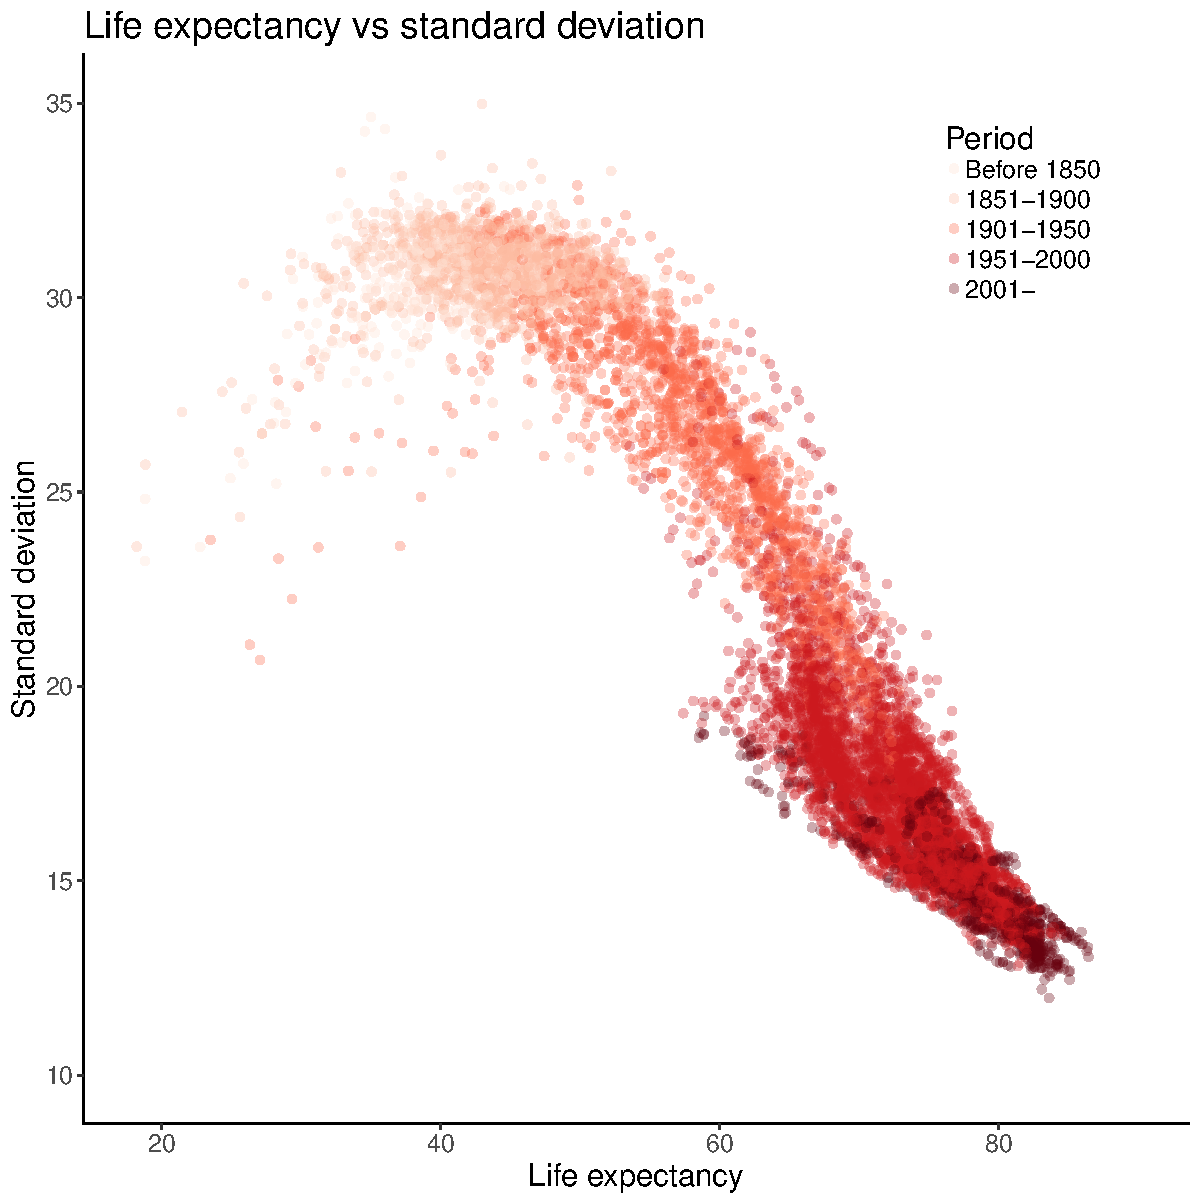
\includegraphics[scale=.4]{Figures/ex_sd}
				\end{center}
			
\end{frame}

\begin{frame}
\begin{center}

		\LARGE{
\textcolor{red}{ What if we take different  \textbf{ages} ? }
\linebreak
\pause
 
\textcolor{blue}{ What if we take different   \textbf{years}? }
\linebreak
\pause


\textbf{We explore with our framework}}

\end{center}			
\end{frame}


\begin{frame}
		
			\begin{center}
		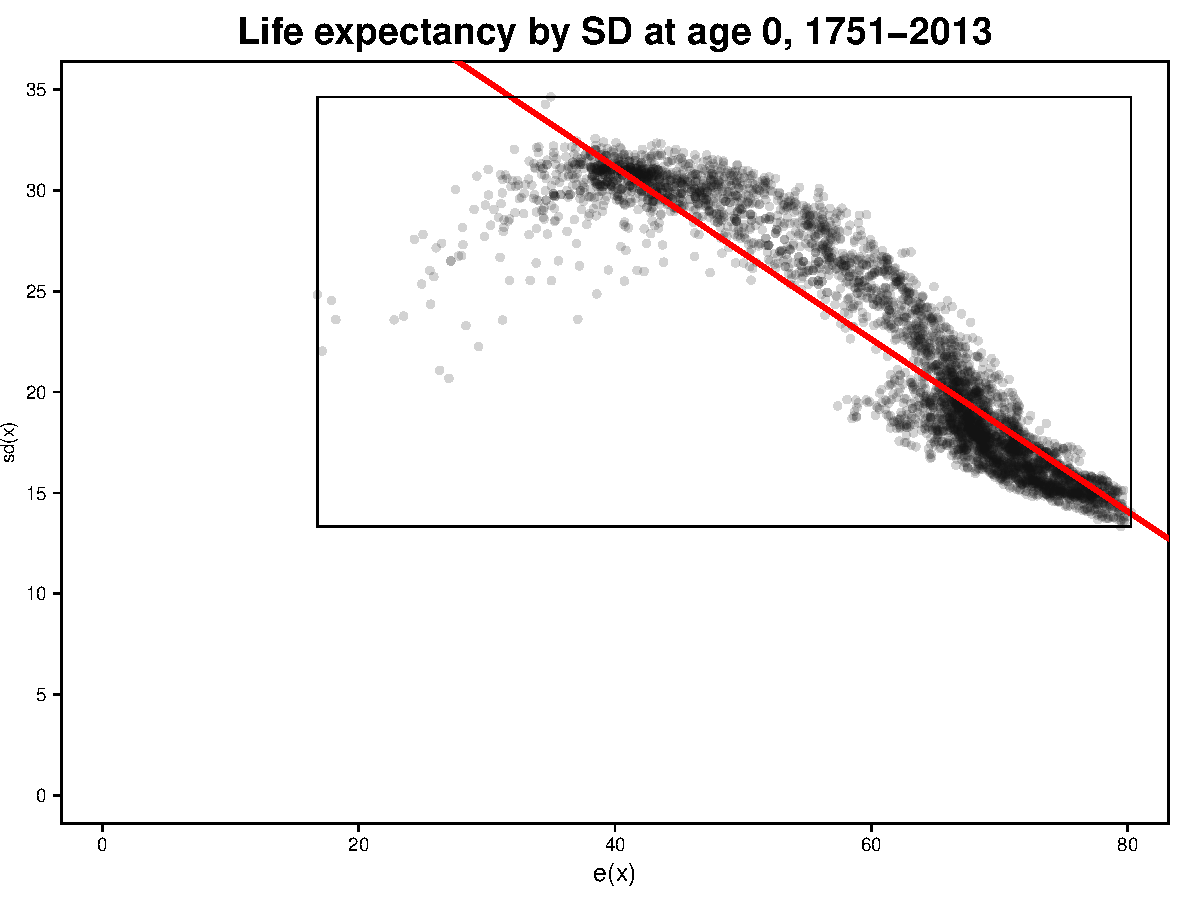
\includegraphics[scale=.53]{Figures/Fig1}
				\end{center}
			
\end{frame}


\begin{frame}
		
			\begin{center}
		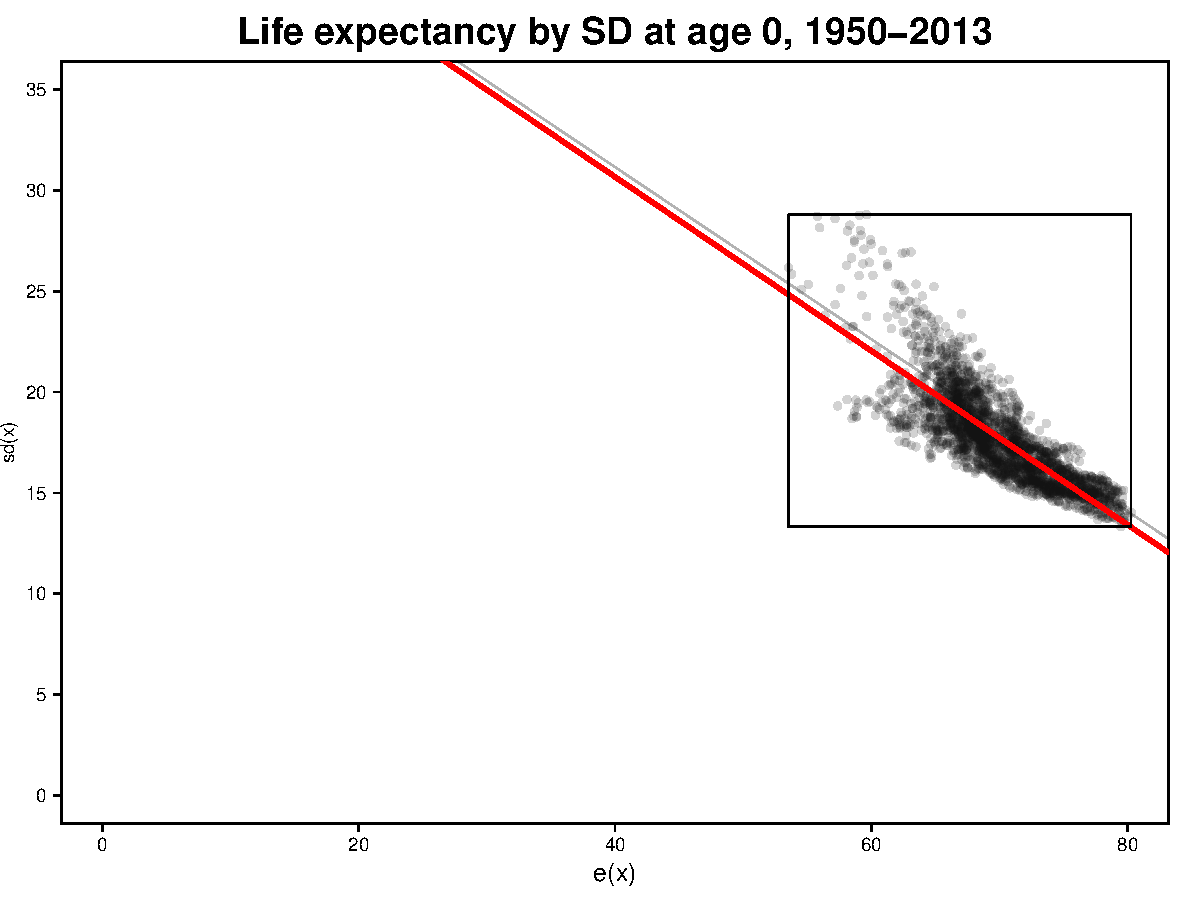
\includegraphics[scale=.53]{Figures/Fig2}
				\end{center}
			
\end{frame}


\begin{frame}
		
			\begin{center}
		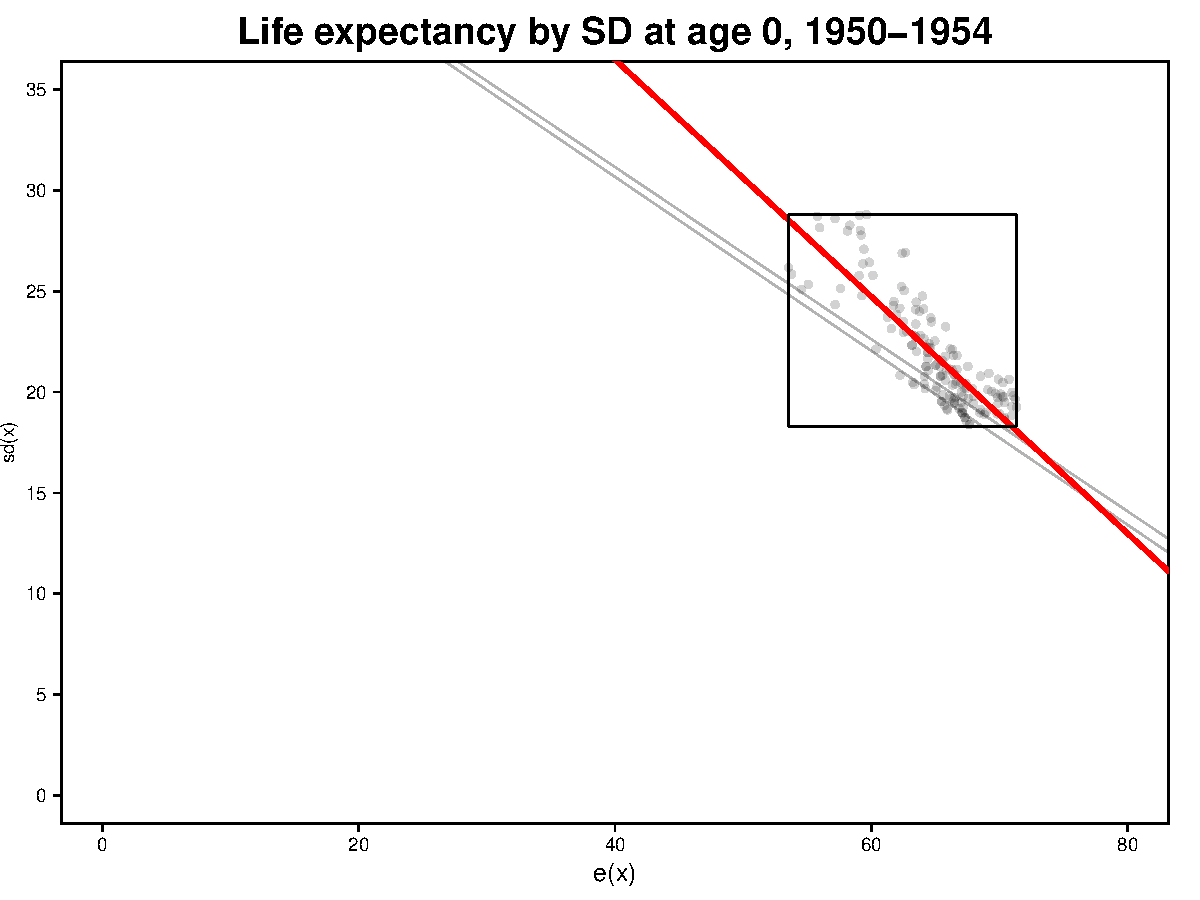
\includegraphics[scale=.53]{Figures/Fig3}
				\end{center}
			
\end{frame}


\begin{frame}
		
			\begin{center}
		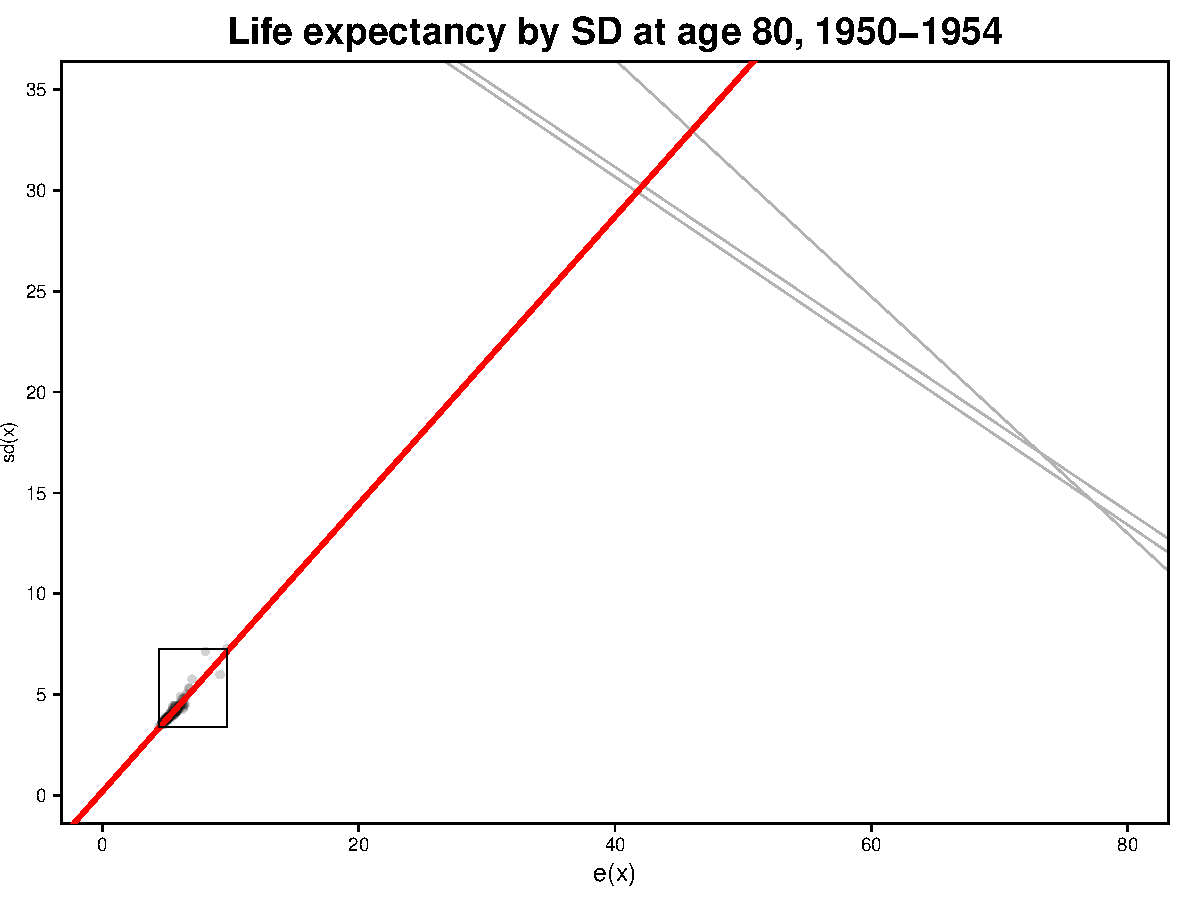
\includegraphics[scale=.53]{Figures/Fig4}
				\end{center}
			
\end{frame}


\begin{frame}
		
			\begin{center}		
\animategraphics[autoplay, loop, scale=0.5]{3}{Figures/Fig5}{1}{21}
				\end{center}
			
\end{frame}

\begin{frame}
		
			\begin{center}		
		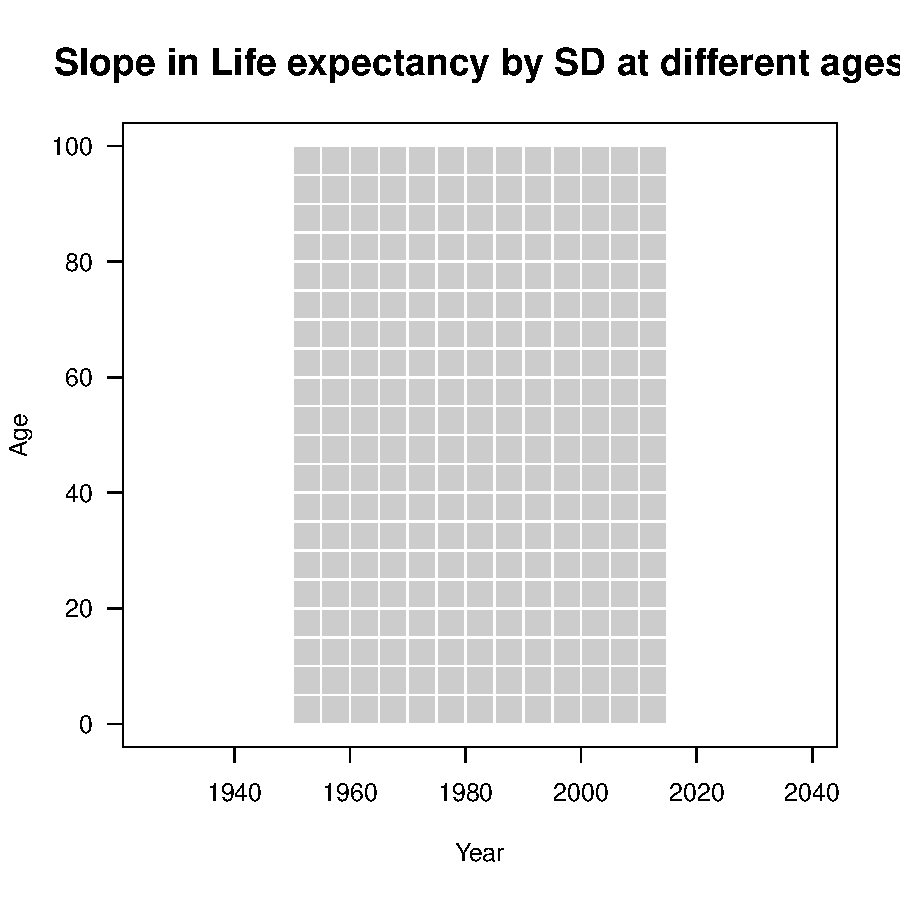
\includegraphics[scale=.53]{Figures/Fig6}
				\end{center}
			
\end{frame}

\begin{frame}
		
			\begin{center}		
		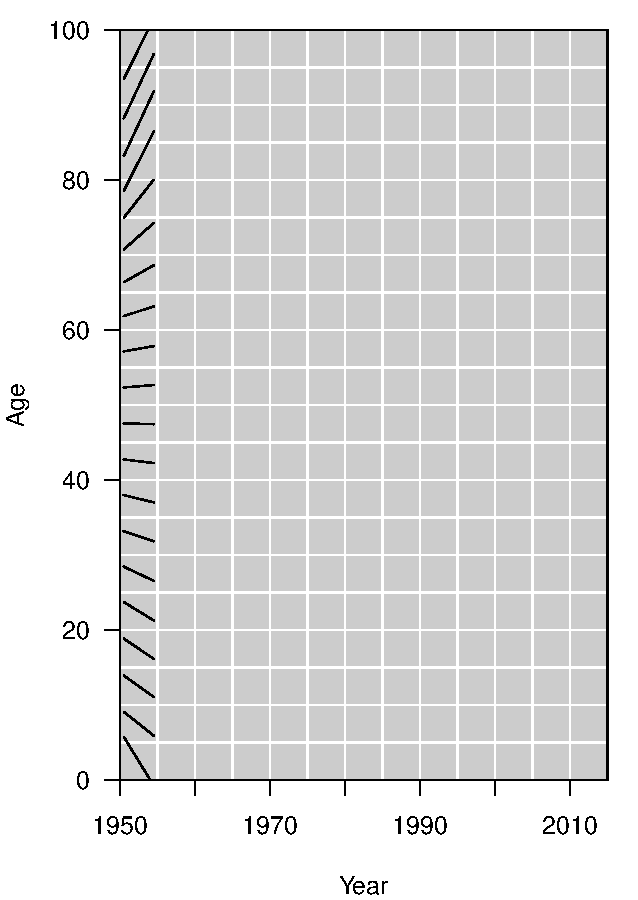
\includegraphics[scale=.53]{Figures/Fig7}
				\end{center}
			
\end{frame}

\begin{frame}
		
			\begin{center}		
		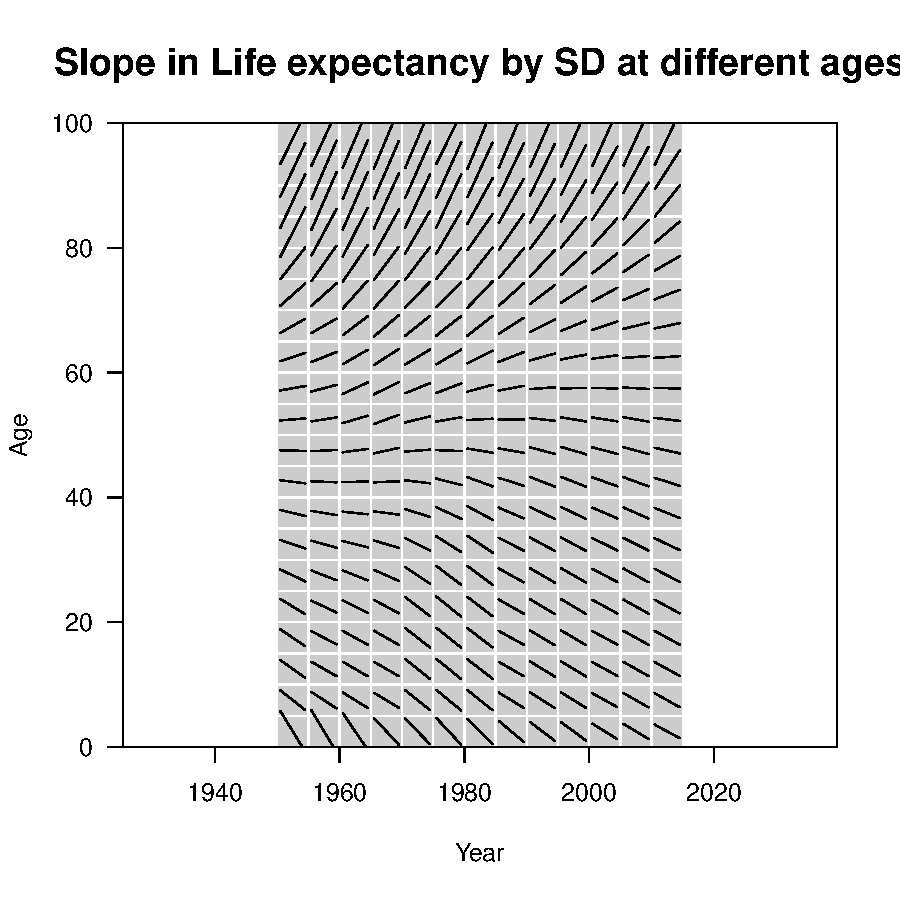
\includegraphics[scale=.53]{Figures/Fig8}
				\end{center}
			
\end{frame}

\begin{frame}
		
			\begin{center}		
		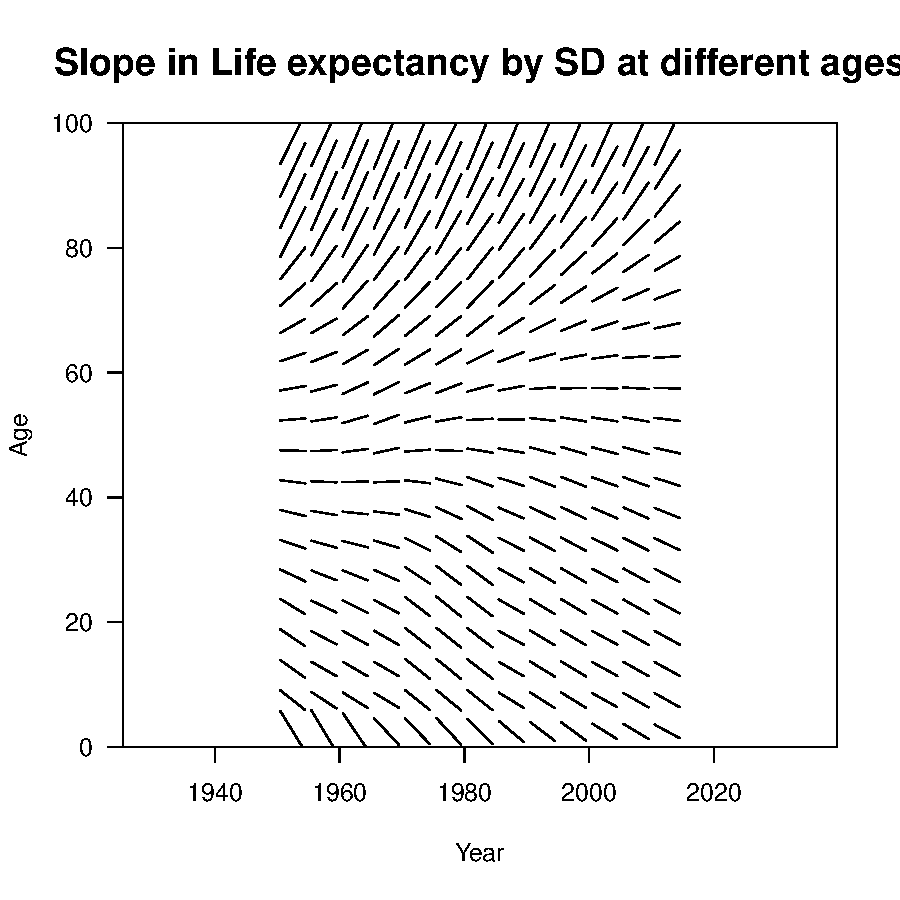
\includegraphics[scale=.53]{Figures/Fig9}
				\end{center}
			
\end{frame}

\begin{frame}
		
			\begin{center}		
		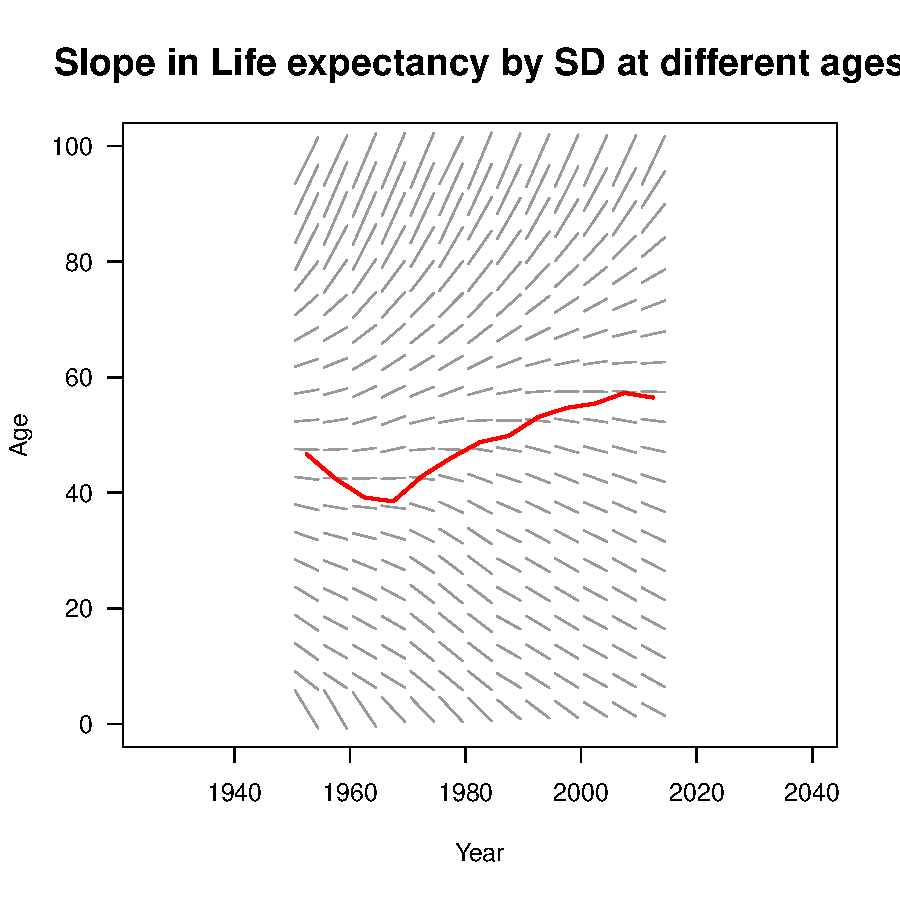
\includegraphics[scale=.53]{Figures/Fig10}
				\end{center}
			
\end{frame}





%%%%%%%%%%%%%%%%%%%%%%%%%%%%%%%%%%%%%%%%%%%%%%%%%%%%%%%%%%%%%%%%%%%%%%%%

%%%%%%%%%%%%%%%%%%%%%%%%%%%%%%%%%%%%%%%%%%%%%%%%%%%%%%%%%%%%%%%%%%%%%%%%
\begin{frame}
 \begin{center}
	\begin{center}
	\Large{
	 \textbf{Go beyond the mean!}}
	\end{center}
	
	\bigskip
	\bigskip
More information: 

jmaburto@health.sdu.dk \quad riffe@demogr.mpg.de

\faTwitter \quad  @jm\_aburto \quad @timriffe1


\faGithub \quad @jmaburto \quad @timriffe


\includegraphics[scale=0.2]{Figures/logos.pdf}    

\end{center}
 
 

\end{frame}



\end{document}
	

